\documentclass{beamer}
\usepackage{../../shared/styles/custom}

\def\checkmark{\tikz\fill[scale=0.4](0,.35) -- (.25,0) -- (1,.7) -- (.25,.15) -- cycle;} 

%\beamerdefaultoverlayspecification{<+->}

	\ifx\relax#1\relax  \item \else \item[#1] \fi
	\abovedisplayskip=0pt\abovedisplayshortskip=0pt~\vspace*{-\baselineskip}}

\title{Unsupervised Learning}
\date{\today}
\author{Nipun Batra}
\institute{IIT Gandhinagar}
\begin{document}
  \maketitle

\begin{frame}Places where you will see unsupervised learning 
\begin{itemize}
\item It can be used to segment the market based on customer preferences.
\item A data science team reduces the number of dimensions in a large dataset to simplify modeling and reduce file size.
\end{itemize}
\end{frame}

\section{Clustering}

\begin{frame}\textbf{REQUIREMENTS:} A predefined notion of similarity/dissimilarity.
\pause
\textbf{Examples:} \\
Market Segmentation: Customers with similar preferences in the same groups. This would aid in targeted marketing.
\end{frame}

\begin{frame}\begin{align*}
WCV\left(C_i\right) &= \frac{1}{|C_i|}__PROTECTED_0__ \\
 WCV\left(C_i\right) &= \frac{1}{|C_i|}\sum_{a\in C_i}\sum_{b\in C_i}|| x_a - x_b ||_2^2
\end{align*}
where $|C_i|$ is the number of points in $C_i$
\end{frame}

\begin{frame}Then,
\begin{align*}
WCV\left(C_i\right) &= \frac{1}{|C_i|}\sum_{a\in C_i}\sum_{b\in C_i}|| x_a - x_b ||_2^2 \\
&= 2\sum_{a\in C_i} ||x_a - x_i||_2^2
\end{align*}
\pause
This shows that K-Means gives the \textbf{local minima}.
\end{frame}

\section{Hierarchal Clustering}

\begin{frame}There is no need to specify $K$ at the start
\pause
\vspace{-0.5cm}
\begin{figure}
        \begin{subfigure}[b]{0.5\textwidth}
                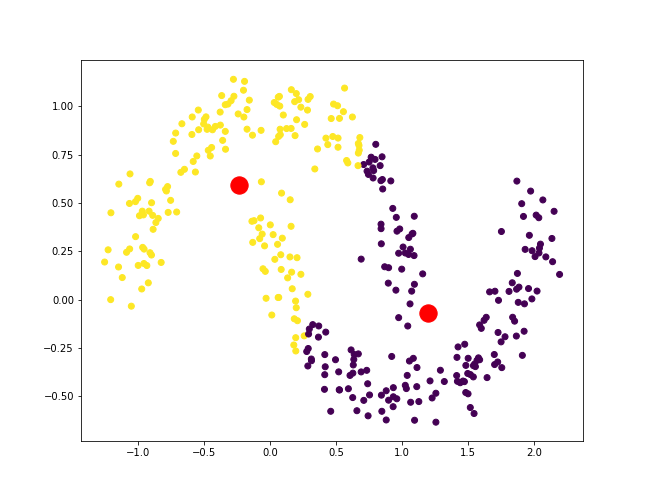
\includegraphics[width=\linewidth]{k_bad_1.png}
        \end{subfigure}%
        \begin{subfigure}[b]{0.5\textwidth}
                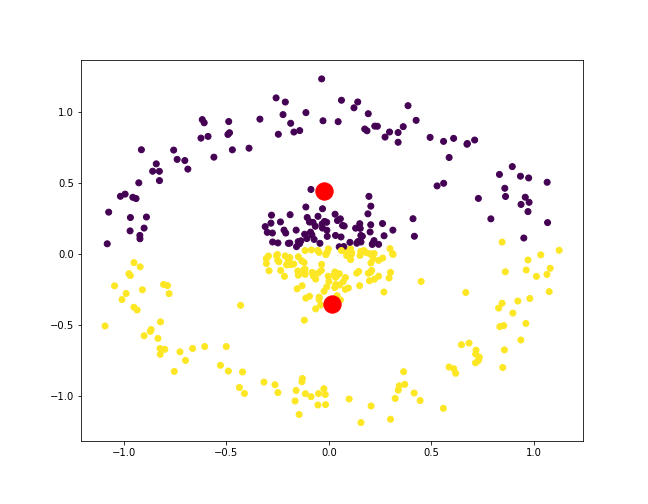
\includegraphics[width=\linewidth]{k_bad_2.png}
        \end{subfigure}%
        \caption{Examples where K-Means fails}
\end{figure}
\end{frame}

\begin{frame}{Algorithm for Hierarchal Clustering}
\vspace{0.5cm}
\begin{enumerate}
\item<1-> Start with all points in a single cluster
\item<4-> Repeat until all points are in a single cluster
\item[]<2-> \begin{enumerate}
\item<2-> Identify the 2 closest points 
\item<3-> Merge them
\end{enumerate}
\end{enumerate}
\vspace{-0.8cm}
\begin{columns}[T]
  \begin{column}{0.5\textwidth}
    \begin{figure}
      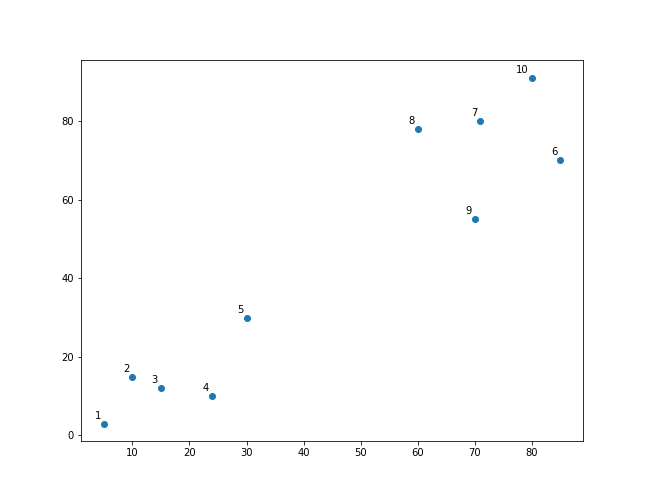
\includegraphics[width=1.1\textwidth]{h_e_1.png}
      \vspace*{-0.6cm}
      \caption{Example Dataset}
    \end{figure}
  \end{column}
  \begin{column}{0.5\textwidth}
    \begin{figure}
    \begin{overprint}
      \onslide<4-> 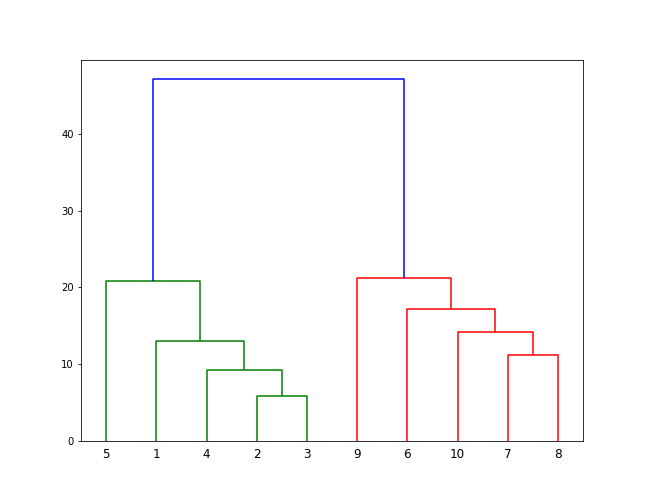
\includegraphics[width=1.1\textwidth]{h_e_2.png}
      \vspace*{-0.6cm}
      \caption{Final Clustering}
    \end{overprint}
    \end{figure}
  \end{column}
\end{columns}
\end{frame}

\begin{frame}{Joining Clusters/Linkages}
\begin{columns}[T]
  \begin{column}{0.33\textwidth}
  \textbf{Complete}\\
  Max inter-cluster similarity
  \end{column}
  \begin{column}{0.33\textwidth}
  \textbf{Single} \\
  Min inter-cluster similarity
  \end{column}
  \begin{column}{0.33\textwidth}
  \textbf{Centroid} \\
  Dissimilarity between cluster centroids 
  \end{column}
\end{columns}

\end{frame}

\begin{frame}{More Code}
\begin{center}
\href{https://colab.research.google.com/drive/1HMPn0mpMAe4XFe5Zvh4oExgi5evkgjTi}{Google Colab Link}
\end{center}
\end{frame}

\end{document}
